\documentclass[handout]{beamer}
\usepackage{beamerthemesplit}
\usepackage{pgfpages}
\usepackage{verbatim}

\usepackage{tikz}
\usetikzlibrary{arrows,%
                shapes,positioning}

\tikzstyle{vertex}=[circle,fill=black!25,minimum size=20pt,inner sep=0pt]
\tikzstyle{selected vertex} = [vertex, fill=red!24]
\tikzstyle{edge} = [draw,thick,-]
\tikzstyle{weight} = [font=\small]
\tikzstyle{selected edge} = [draw,line width=5pt,-,red!50]
\tikzstyle{ignored edge} = [draw,line width=5pt,-,black!20]

\newcommand{\field}[1]{\mathbb{#1}} %requires amsfonts

\usetheme{Antibes}
\usecolortheme{beaver}
\title[Optimizing Diffusion and Confusion]{Optimizing Diffusion and Confusion \\ in Cryptographic Primitives}

\usepackage{mathptmx}
\usepackage[scaled=.90]{helvet}
\usepackage{courier}
\usepackage[T1]{fontenc}

%\pgfpagesuselayout{4 on 1}[letterpaper,border shrink=5mm]

\institute[RIT]{}
\date{\today}
%\subtitle{}
\author{Christopher A. Wood}
%\institute[]{}
\date{May 9, 2012}
\begin{document}

%%%%%
%%
%% Resource link: http://www.math-linux.com/spip.php?article77
%%
%%%%

\begin{frame}
	\titlepage
\end{frame}

\begin{frame}
	\frametitle{Agenda}
	\tableofcontents
\end{frame}

\section{Cryptographic algorithm security fundamentals}
\begin{frame}
	\frametitle{Algorithm security fundamentals}
	\begin{itemize}
		\item Strive for high confusion and diffusion
		\begin{itemize}
			\item \emph{Confusion} - complex relationship between the secret key and ciphertext
			\item \emph{Diffusion} - dissipation of plaintext bits throughout ciphertext bits
		\end{itemize}
	\end{itemize}
\end{frame}

\begin{frame}
	\frametitle{Algorithm construction principles}
	\begin{itemize}
		\item Algorithms are composed of a combination of linear and nonlinear operations
		\item Maximize diffusion through linear transformations
		\begin{itemize}
			\item Linear permutations
			\item Circular shifts
			\item Modular addition 
		\end{itemize}
		\item Maximize confusion through nonlinear operations
		\begin{itemize}
			\item S(ubstitution)-box (Rijndael cipher)
			\item Add-Rotate-XOR (ARX) combination functions (Threefish cipher)
			\item Discrete-time difference equations (often defined as recurrence relations)
		\end{itemize}
	\end{itemize}
\end{frame}

\begin{frame}
	\frametitle{Measuring security}
	\begin{itemize}
		\item Linear behavior
		\begin{itemize}
			\item Exhibit avalanche effect and adherence to Strict Avalanche Criterion (SAC)
		\end{itemize}
		\item Nonlinear behavior
		\begin{itemize}
			\item Branch number
			\item Direct measurement of nonlinear behavior
		\end{itemize}
	\end{itemize}
\end{frame}

\begin{frame}
	\frametitle{Avalanche effect}
A function $f : \field{F}_2^n \to \field{F}_2^n$ exhibits the \emph{avalanche effect} if and only if 
	\begin{eqnarray*}
		\sum_{x \in \field{F}_2^n} \text{wt}(f(x) \oplus f(x \oplus c_{i}^{n})) = n2^{n-1},*
	\end{eqnarray*}
	for all $i (1 \leq i \leq n)$, where $c_{i}^{n} = [0, 0, ..., 1, ..., 0]$ (where a $1$ is in the $n$th position of the vector of cardinality $n$). \\
	%\vspace{0.25cm}
	%This is a significantly stronger sufficient condition for high measures of diffusion.\\
	\vspace{0.25cm}
	*\emph{wt} indicates the Hamming Weight function
\end{frame}

\begin{frame}
	\frametitle{SAC}
	A function $f : \field{F}_2^n \to \field{F}_2^n$ satisfies the \emph{Strict Avalanche Critertion (SAC)} if for all $i (1 \leq i \leq n)$ the following equations hold:
	\begin{eqnarray*}
		\sum_{x \in \field{F}_2^n} f(x) \oplus f(x \oplus c_i^n) = (2^{n-1}, 2^{n-1}, ..., 2^{n-1})
	\end{eqnarray*}
	This simply means that $f(x) \oplus f(x \oplus c_i^n)$ is balanced for every element in $\field{F}_2^n$ with Hamming distance of $1$. 
\end{frame}

%TODO: include image of avalanche effect

\begin{frame}
	\frametitle{Branch number}
	The \emph{branch number} of an $n \times n$-bit S-Box is
	\begin{eqnarray*}
		BN = \text{min}_{a, b\not=a}(\text{wt}(a \oplus b) + \text{wt}(S(a) \oplus S(b))),
	\end{eqnarray*}
	where $a, b \in \field{F}_2^n$.
\end{frame}

%TODO: include another slide about branch number (with different definition?)

\begin{frame}
	\frametitle{S-box specific nonlinear measurements}
	The nonlinearity of an $n \times n$-bit S-Box from $\field{F}_2^n \to \field{F}_2^n$ can be measured by
	\begin{eqnarray*}
		P_S = \text{max}_{0 \not= a, b}|\{x \in \field{F}_2^n : S(x + a) - S(x) = b\}|
	\end{eqnarray*}
	where $a, b \in \field{F}_2^n$.
\end{frame}

%\begin{frame}
%	\frametitle{Walsh transformation measurement}
%	\begin{itemize}
%		\item TODO
%	\end{itemize}
%\end{frame}

\section{Design Criteria}
\begin{frame}
	\frametitle{Implementation Considerations}
	\begin{itemize}
		\item Design against common cryptanalysis techniques
		\item Linear transformations
		\begin{itemize}
			\item Linear permutations
			\item Circular shifts
			\item Modular addition
		\end{itemize}
		\item Nonlinear transformations
		\begin{itemize}
			\item S-boxes
			\item ARX functions
			\item Chaotic recurrence relations
			%\item Number theoretic PRNGs
		\end{itemize}
	\end{itemize}
\end{frame}

\begin{frame}
	\frametitle{S-boxes}
	\begin{itemize}
		\item Bijective functions from $\field{F}_2^n \to \field{F}_2^n$.
		\item Designed for optimal nonlinearity and algebraic complexity.
		\begin{itemize}
			\item Maximize the avalanche property of the S-box for all input/output pairs.
			\item Minimize the differential propagation probability %TODO: make sure this is known
			\item Maximize complexity of the algebraic expression for the S-box in $\field{F}_2^n$
		\end{itemize}
	\end{itemize}
\end{frame}

\begin{frame}
	\frametitle{Rijndael Substitute Bytes Calculation}
	Rijndael sub-bytes affine transformation
	\begin{center}
      		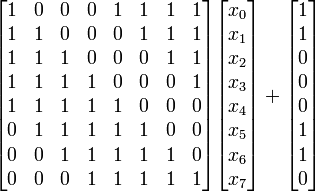
\includegraphics[width=70mm]{images/rijndael_sub_affine.png}
	\end{center}
\end{frame}

\begin{frame}
	\frametitle{Rijndael Substitute Bytes Calculation}
	This affine can also be represented algebraically as follows
	\begin{eqnarray*}
		b_i' = b_i \oplus b_{(i+4) mod 8} \oplus b_{(i+5) mod 8} \oplus b_{(i+6) mod 8} \oplus b_{(i+7) mod 8} \oplus c_i
	\end{eqnarray*}
	where $i$ is the $i$th bit of the input byte $b$ and $c = \langle 01100011 \rangle$.
\end{frame}

%TODO: another slide on S-boxes
\begin{frame}
	\frametitle{S-boxes}
	\begin{itemize}
		\item Random and fixed structure (i.e. Rijndael s-box) designs have been propsed based on susceptibility to differential cryptanalysis
		\begin{itemize}
			\item Fixed structure are more beneficial for security analysis and proof purposes
		\end{itemize}
		\item Various construction criterias have been proposed
		\begin{itemize}
			\item Nydberg (91) - \emph{"A perfect nonlinear S-box is a substitution transformation with evenly distributed directional derivatives."}
			\item Dawson and Tavares (91) - static and dynamic criteria supporting claim for high branch numbers and avalanche property
			\item ...
		\end{itemize}
	\end{itemize}
\end{frame}

\begin{frame}
	\frametitle{Provable Security for S-boxes}
	\textbf{Theorem: } (KN Theorem) It is assumed that in a DES-like cipher with $f :  \field{F}_2^m \to  \field{F}_2^n$ (the substitution function) the keys are independent and uniformly random. Then, the probability of an s-round differential, $s \geq 4$, is less than or equal to $p_{max}^2$, where $p_{max}$ is defined in terms of the nonlinearity of the S-box as follows:
	\begin{eqnarray*}
		p_{max} \leq max_{b} max_{a \not= 0} Pr[f(Y + a) + f(a) = b],
	\end{eqnarray*}
	where $a, b \in \field{F}_2^n$.
	% How valid is the random key distribution assumption?
	% Y is some other element in the field... just go back to nonlinearity example
\end{frame}

\begin{frame}
	\frametitle{Similar Nonlinear Functions}
	\begin{itemize}
		\item Bent functions
		\item Vector bent functions
		\item APN S-boxes
		\item Differentially Uniform $\delta$-Uniform S-box functions
		\item ...
	\end{itemize}
\end{frame}

%http://fse2012.inria.fr/SLIDES/kaisa.pdf
\begin{frame}
	\frametitle{Bent Functions}
	The correlation between a Boolean function $f : \field{F}_2^n \to \field{F}_2$ and a linear function $x \mapsto u \cdot x$ is defined as
	\begin{eqnarray*}
	c_f(u) = \frac{1}{2^n}(|\{x \in \field{F}_2^n : f(x) = u \cdot x\} - |\{x \in \field{F}_2^n : f(x) \not= u \cdot x\})
	\end{eqnarray*}
	A Boolean function is thus called \emph{bent} if
	\begin{eqnarray*}
		|c_f(u)| = 2^{\frac{-n}{2}},
	\end{eqnarray*}
	for all $u \in \field{F}_2^n$. Note that $n$ must be even in order for $f$ to be bent.
\end{frame}

\begin{frame}
	\frametitle{Vector Bent Functions}
	\begin{itemize}
		\item Perfect nonlinearity of Boolean functions strongly correlates to cryptographic strength
		\item Nydberg's "perfect nonlinear functions" - an multiple dimension Boolean functions
	\end{itemize}
	A vector function $f : \field{F}_2^n \to \field{F}_2^m$ is said to be \emph{bent} if
	\begin{itemize}
		\item $w \cdot f$ is bent for all $w \not= 0$.
		\item $f$ is perfect nonlinear ($f(x + \alpha) = f(x)$ is uniformly distributed as $x$ varies, for all fixed $\alpha \in \field{F}_2^n - \{0\}$.
	\end{itemize}
\end{frame}

\begin{frame}
	\frametitle{APN S-boxes}
	A function $f : \field{F}_2^n \to \field{F}_2^n$ is said to be \emph{almost perfect nonlinear} (APN) if
	\begin{eqnarray*}
		|\{x : f(x + \alpha) + f(x) = \beta\}| \leq 2,
	\end{eqnarray*}
	for all fixed $\alpha \in \field{F}_2^n - \{0\}$. Some examples include:
	\begin{itemize}
		\item $f : \field{F}_2^n \to \field{F}_2^n, f(x) = x^3$
		\item $f : \field{F}_2^n \to \field{F}_2^n, f(x) = x^{2k + 1}$ (i.e. any odd power exponent)
	\end{itemize}
\end{frame}

\begin{frame}
	\frametitle{Differentially $\delta$-Uniform S-box functions}
	A function $f : \field{F}_2^n \to \field{F}_2^n$ is said to be \emph{differentially $\delta$-uniform} if
	\begin{eqnarray*}
		|\{x : f(x + \alpha) + f(x) = \beta\}| \leq \delta,
	\end{eqnarray*}
	Small values for $\delta$ are desirable - indicates higher degree of nonlinearity.
\end{frame}

\begin{frame}
	\frametitle{ARX functions}
	\begin{itemize}
		\item Nonlinear functions consisting of a combination of modular addition, bitwise rotation, and bitwise XOR operations
		\item Analysis of differential propagation is difficult
		\begin{itemize}
			\item Differential properties of sub-operations need to be considered (adp$^{\oplus}$, xdp$^{+}$)
		\end{itemize}
		\item Most susceptible to rotational cryptanalysis
		\begin{itemize}
			\item Threefish was attacked using a combination of rotational cryptanalysis with a rebound attack (Khovratovich et al, 2010) - led to adjustment of Threefish rotation constants %rotational crypt can essentially be thought of as DC but treating pairs of words as (unrotated, rotated) and looking at p(rotate(x+y) == rotate(X) + rotate(y))
		\end{itemize}
	\end{itemize}
\end{frame}

%TODO: another slide and MORE details on ARX functions - see Threefish paper?
%\begin{frame}
%	\frametitle{ARX functions}
%	\begin{itemize}
%		\item 
%	\end{itemize}
%\end{frame}

\begin{frame}
	\frametitle{Chaotic recurrence relations}
	\begin{itemize}
		\item Chaotic systems are defined by:
		\begin{itemize}
			\item Sensitivity to initial conditions 
			\item Topologically mixing (i.e. covers entire state space)
			\item Dense (and long) periodic orbits 
		\end{itemize}
		\item Some recurrence relations exhibit "chaotic" behavior (e.g. the Logistic Map)
	\end{itemize}
	\begin{eqnarray*}
		x_{n+1} = rx_{n}(1 - (x_{n}))
		\label{logisticmap}
	\end{eqnarray*}
\end{frame}

\begin{frame}
	\frametitle{Chaos in the Logistic Map}
	\begin{center}
      		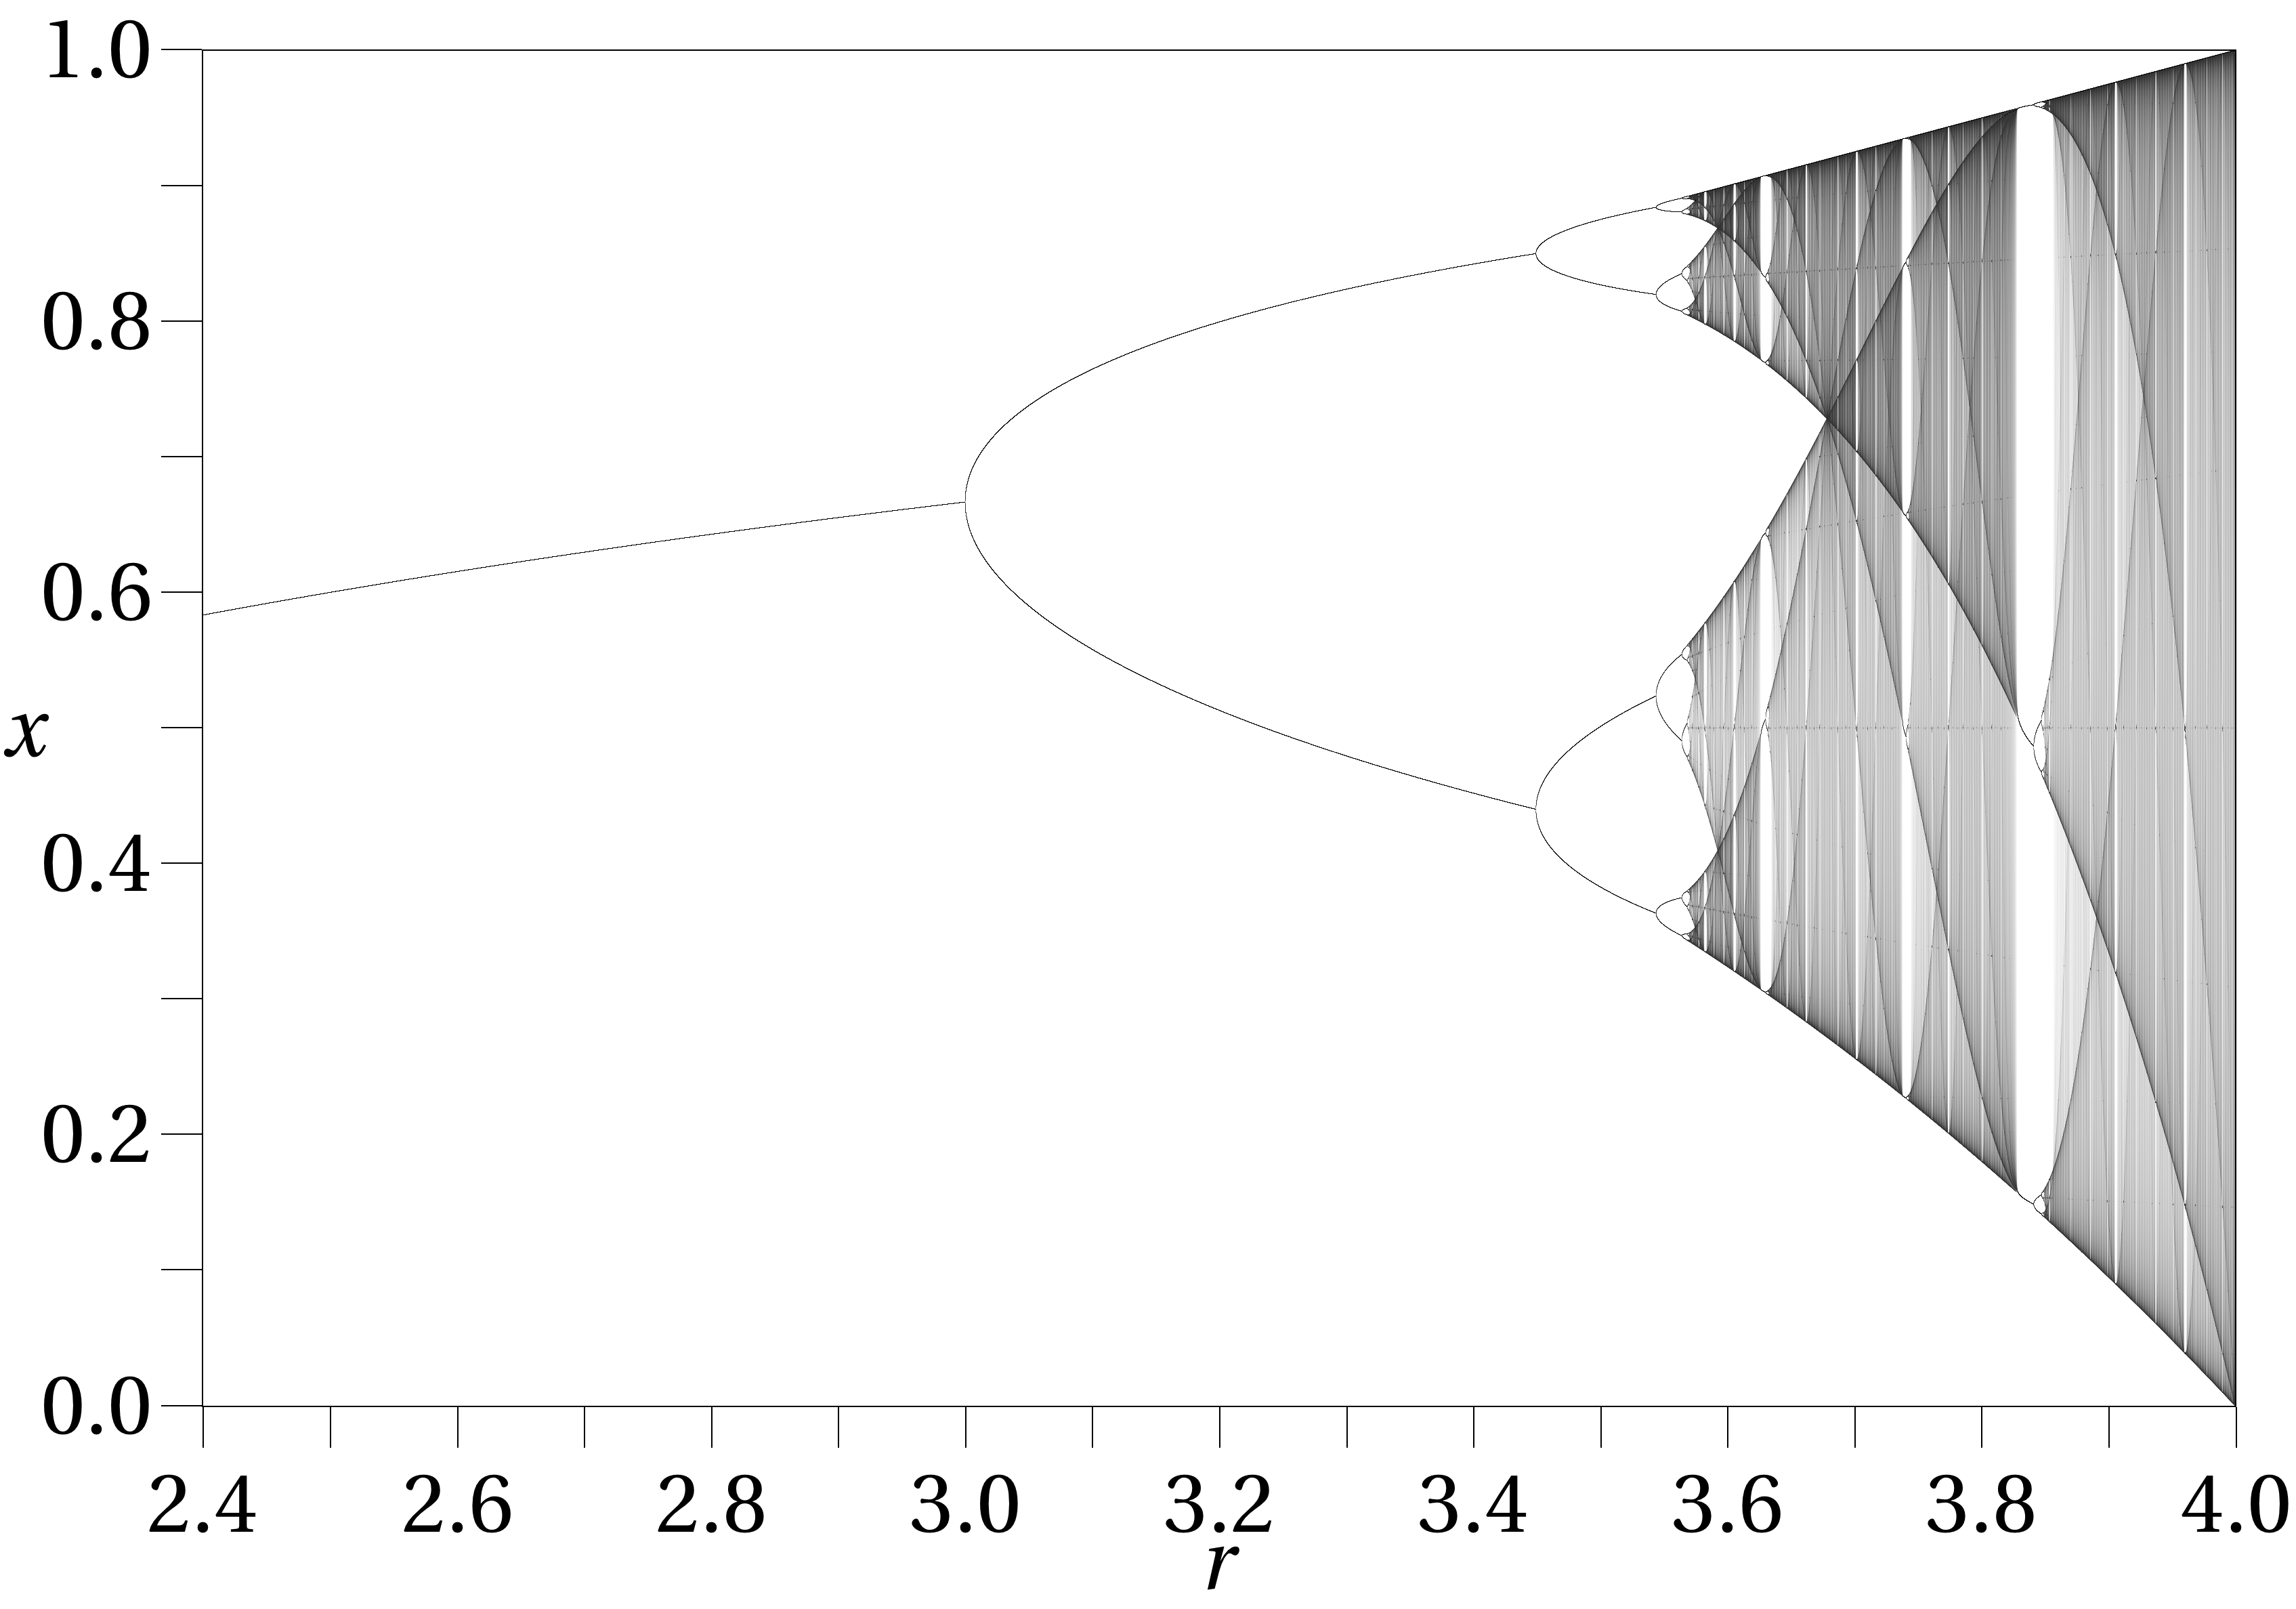
\includegraphics[width=90mm]{images/logistic_bifurcation.png}
	\end{center}
\end{frame}

\section{Case study: Rijndael}
\begin{frame}
	\frametitle{Case Study: Rijndael}
	\begin{itemize}
		\item Four main operations
		\begin{itemize}
			\item Add round key
			\item Shift rows
			\item Substitute bytes
			\item Mix columns
		\end{itemize}
	\end{itemize}
\end{frame}

% ARK: the actual encryption stage, XOR state matrix with appropriate key block in key schedule
% Implications: How much can we guarantee about the construction of the key schedule? Implies there are good and bad keys that can be used. The algorithm should not have to worry about the usage of a "good" key to be secure.
\begin{frame}
	\frametitle{Add Round Key}
	\begin{center}
      		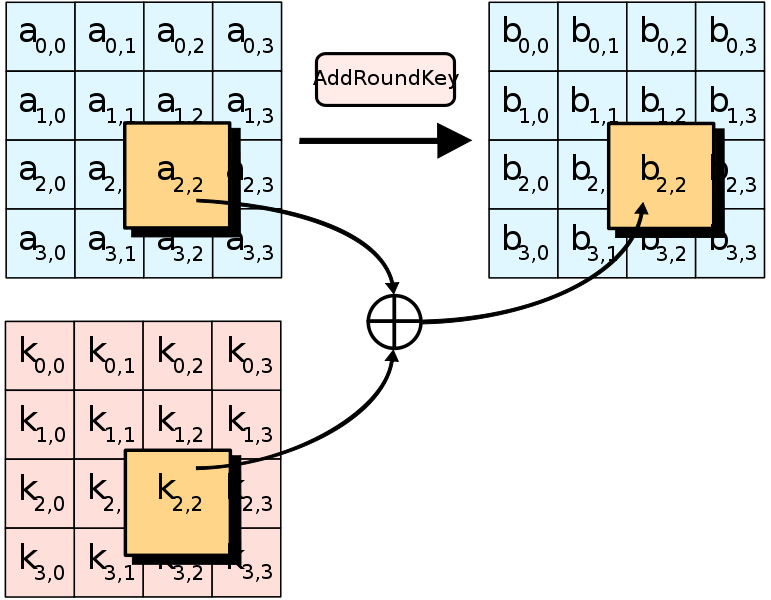
\includegraphics[width=75mm]{images/ark.png}
	\end{center}
\end{frame}

% purpose: just another permutation for diffusion... just rotate the data to avoid linear cryptanalysis. nothing special
\begin{frame}
	\frametitle{Shift Rows}
	\begin{center}
      		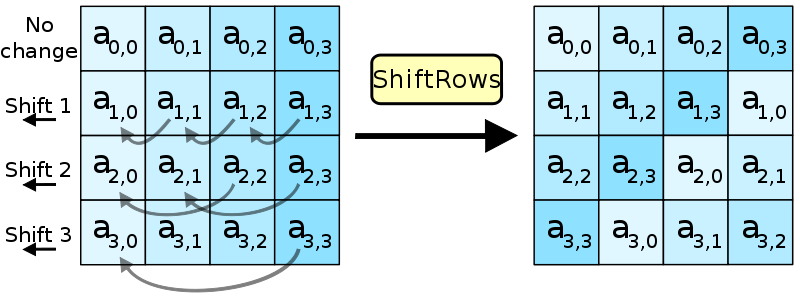
\includegraphics[width=75mm]{images/shift.png}
	\end{center}
\end{frame}

\begin{frame}
	\frametitle{Substitute Bytes} %guarantees about branch number (# of active s-boxes) and the measure of nonlinearity 
	\begin{center}
      		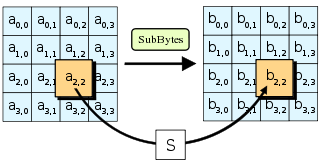
\includegraphics[width=75mm]{images/sub.png}
	\end{center}
\end{frame}

% TODO: mention usage of different MDS matrices
\begin{frame}
	\frametitle{Mix Columns}
	\begin{center}
      		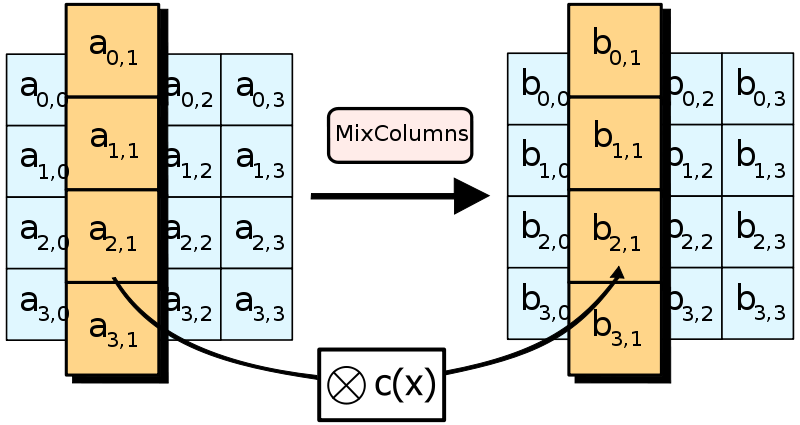
\includegraphics[width=75mm]{images/mix.png}
	\end{center}
\end{frame}

\begin{frame}
	\frametitle{Mix Columns MDS Matrix}
	\begin{center}
      		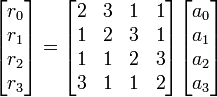
\includegraphics[width=75mm]{images/mix_ops.png} %MDS matrix used for diffusion (why 4x4? other larger wide-pipe designs have been propsed, including 8x8 and 16x16)
	\end{center}
\end{frame}

\section{Open problems and future work}
\begin{frame}
	\frametitle{Open problems and future work}
	\begin{itemize}
		\item Diffusion and confusion are the determining factors of secure primitives
		\pause
		\item The design space for diffusion and confusion layers is not exhausted
		\begin{itemize}
			\item Other compositions of discrete mathematical objects and operations exist (bent functions, MDS matrices, etc)
			\item Can they provide the same measure of security as existing objects (i.e. S-boxes, ARX functions)?
		\end{itemize}
		\pause
		\item How feasible is the reduction of the security of block ciphers to an multivariate optimization problem?
		\item How different are the implementation aspects of each of these mathematical objects?
		\begin{itemize}
			\item Can we improve existing implementations?
		\end{itemize}
	\end{itemize}
\end{frame}

%TODO: insert slides about optimization concept slides here
%1. Include work done by Julia
%2. Mention some common optimization techniques
%3. mention idea of representing state as multivariate polynomial equation

%TODO: insert slides about implementation details here
%simply include some common implementation techniques, broken up by HW and SW
%discuss some of the latest works relating to optimization techniques

\end{document}
